This chapter presents an IMP solution which solves issues of user profile-based identity management by enabling users to create, manage, and access user profiles through IMP. For the utilization of IMP services as described by the IMP solution, an integration architecture is presented that enables the OZG system architecture described in section 2.2 to access the IMP system described in section 2.1.

\begin{figure}[h]
    \centering
    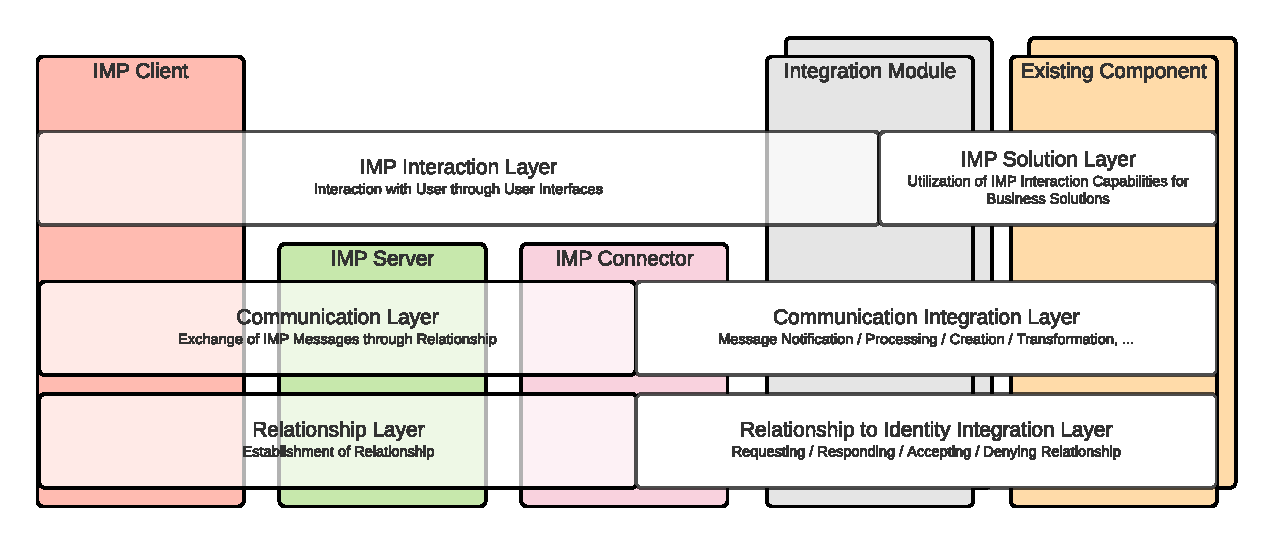
\includegraphics[scale=0.6]{Diagrams/Integration Architecture 1/IMP Layer Diagram Integration.pdf}
    \caption{IMP System Layers}
    \label{integration1:layer_diagram}
\end{figure}

As shown in figure \ref{integration1:layer_diagram}, the integration takes place on three layers:

\paragraph{IMP Solution Layer} 
The IMP solution is integration on the use case level. It presents possibilities of leveraging the interaction capabilities of the IMP system in the context of the Service Provider for the improvement of usability, data protection and security. Furthermore, it describes which types of relationships the Service Provider can use in their business scenario, how relationships can be processed, which types of messages can be exchanged through the relationships, what the purpose of each message can be and how the IMP client can react to different message types.

\paragraph{Technological Integration} 
The Technological Integration is integration on the system level. It consists of an integration architecture enabling the existing systems of the Service Provider to utilize the IMP system as described by the IMP solution. The Technological Integration is separated into a "Communication Integration Layer" and a "Relationship to Identity Integration Layer". On the "Relationship to Identity Integration Layer" the integration architecture enables the existing systems to create relationship templates and establish relationships. On the "Communication Integration Layer" it enables the existing systems to send and receive different types of IMP messages.

\section{IMP Solution Integration}

\subfile{10-imp_solution_integration}

\section{Technological Integration}

\subfile{11-technological_integration}